\documentclass[12pt, twoside]{article}
\usepackage[letterpaper, margin=1in, headsep=0.2in]{geometry}
\setlength{\headheight}{0.6in}
%\usepackage[english]{babel}
\usepackage[utf8]{inputenc}
\usepackage{microtype}
\usepackage{amsmath}
\usepackage{amssymb}
%\usepackage{amsfonts}
\usepackage{siunitx} %units in math. eg 20\milli\meter
\usepackage{yhmath} % for arcs, overparenth command
\usepackage{tikz} %graphics
\usetikzlibrary{quotes, angles}
\usepackage{graphicx} %consider setting \graphicspath{{images/}}
\usepackage{parskip} %no paragraph indent
\usepackage{enumitem}
\usepackage{multicol}
\usepackage{venndiagram}

\usepackage{fancyhdr}
\pagestyle{fancy}
\fancyhf{}
\renewcommand{\headrulewidth}{0pt} % disable the underline of the header
\raggedbottom
\hfuzz=2mm %suppresses overfull box warnings

\usepackage{hyperref}

\fancyhead[LE]{\thepage}
\fancyhead[RO]{\thepage \\ Name: \hspace{4cm} \,\\}
\fancyhead[LO]{BECA / Dr. Huson / Geometry\\*  Unit 8: Year-to-date Regents review\\* 3 March 2023}

\begin{document}

\subsubsection*{8.6 Quiz: Triangle angles, transversals, segments, solids}
\begin{enumerate}
\item What is the sum of the internal angle measures of a triangle?
\begin{multicols}{2}
\begin{enumerate}
  \item $45^\circ$
  \item $90^\circ$
  \item $120^\circ$
  \item $180^\circ$
\end{enumerate}
\end{multicols}

\item Given $\triangle ABC$ with $\overrightarrow{ACD}$.
\begin{center}
  \begin{tikzpicture}[scale=0.7]
  \draw [thick, <-]
  (10,0)node[below]{$D$}--
  (0,0)node[below]{$A$}--
  (4,4)node[above]{$B$}--
  (7,0)node[below]{$C$};
  \node at (0.9,0.4){1};
  \node at (6.2,0.4){3};
  \node at (7.2,0.4){4};
  \node at (4,3.3){2};
\end{tikzpicture}
\end{center}
Which equation is always true?
\begin{multicols}{2}
\begin{enumerate}
  \item $m\angle 3 = m\angle 1 + m\angle 2$
  \item $m\angle 3 = m\angle 1 - m\angle 2$ 
  \item $m\angle 4 = m\angle 1 + m\angle 2$
  \item $m\angle 4 = m\angle 3 - m\angle 2$
\end{enumerate}
\end{multicols}

\item A regular hexagon is rotated about its center. Which degree measure will carry the regular hexagon onto itself? 
\begin{multicols}{2}
\begin{enumerate}
  \item $45^\circ$
  \item $60^\circ$
  \item $90^\circ$
  \item $135^\circ$
\end{enumerate}
\end{multicols}

\item Two parallel lines intersect a transversal. Given corresponding angles  m$\angle 1 = 3x+18$ and m$\angle 2 = 5x-50$. What is the value of $x$?
\begin{multicols}{2}
  \begin{enumerate}
    \item $34^\circ$
    \item $42^\circ$
    \item $45^\circ$
    \item $51^\circ$
  \end{enumerate}
  \begin{tikzpicture}[scale=1]
    \draw [<->, thick] (3,0)--(8.5,0);
    \draw [<->, thick] (2.5,2)--(8,2);
    \draw [<->, thick] (5,-1)--(3,3);
    \node at (5.3, 2.25){m$\angle 1 = 3x+18$};
    \node at (6.1, 0.25){m$\angle 2 = 5x-50$};
  \end{tikzpicture}
  \end{multicols}

\newpage
\item What is the midpoint of $\overline{AB}$, with $A(2,-2)$ and $B(6,12)$.
\begin{multicols}{2}
  \begin{enumerate}
    \item $(0,9)$
    \item $(9,0)$
    \item $(5,4)$
    \item $(4,5)$
  \end{enumerate}
  \end{multicols} \vspace{1cm}

\item Point $G$ divides $\overline{AB}$ so that $AG:GB = 1:2$. If $A$ has coordinates $(1,0)$ and $B$ has coordinates $(7,9)$, what are the coordinates of $G$?
\begin{multicols}{2}
  \begin{enumerate}
    \item $(3,3)$
    \item $(4,4.5)$
    \item $(5,6)$
    \item $(8,0.5)$
  \end{enumerate}
  \end{multicols} \vspace{2cm}

\item What is the volume of a rectangular prism with length 3 cm, width 4 cm, and height 5 cm to the nearest cubic centimeter? 
\begin{multicols}{2}
  \begin{enumerate}
    \item $12$
    \item $55$
    \item $60$
    \item $90$
  \end{enumerate}
  \end{multicols} \vspace{0.5cm}

\item A square tabletop will be made of oak wood that weighs 0.025 pounds per cubic inch. The tabletop will measure 48 inches on each side and is two inches thick. Determine the weight of the tabletop, to the nearest pound.
\begin{multicols}{2}
  \begin{enumerate}
  \item $39$
  \item $98$
  \item $115$
  \item $133$
\end{enumerate}
\end{multicols} \vspace{3cm}

\item If a right triangle is continuously rotated around one of its legs (not the hypotenuse), what is the three-dimensional figure formed?
  \begin{multicols}{2}
  \begin{enumerate}
    \item cone
    \item sphere
    \item cylinder
    \item rectangular prism
  \end{enumerate}
\end{multicols}


\end{enumerate}
\end{document}